% LSQR recursion follows Paige and Saunders, ACM TOMS 8 (1982), Algorithm LSQR.
% LSMR recursion checked against Fong and Saunders, SIAM J. Sci. Comput. 33 (2011), Algorithm LSMR.
\subsection{Golub--Kahan双对角化}
\label{sec:ls-bidiagonal-iteration}

\subsubsection{主要思想}

对一般的$\bm A\in\mathbb R^{m\times d}$，残差在$m$维的数据空间，未知量在$d$维空间，不能像方阵那样反复乘$\bm A$；把数据空间的向量送回未知量空间的是$\bm A^\top$。Golub--Kahan双对角化因此交替作用$\bm A$与$\bm A^\top$，在数据空间建立标准正交基$\bm u_1,\bm u_2,\ldots$，在未知量空间建立与之配对的标准正交基$\bm v_1,\bm v_2,\ldots$。在这两组基下，$\bm A$只剩两条对角线上的系数，长方矩阵问题被压缩成一个下双对角的小问题。它是后面LSQR和LSMR共用的内部过程，基向量和双对角系数只是求解器的中间状态，不作为输出。

\subsubsection{算法实现}

\paragraph{起步}
输入仍是$\bm A$与$\bm b\in\mathbb R^m$。后面两种求解器都固定零初值$\bm x_0=\bm0$，这是本节选出最小范数解的约定；生成多少步由求解器的步数上限$K$控制。起步先处理右端：若$\bm b=\bm0$，零向量就是最小范数解，直接输出。否则令
\[
 \beta_1=\lVert\bm b\rVert_2,\quad \bm u_1=\bm b/\beta_1,\quad
 \bm q=\bm A^\top\bm u_1,\quad \alpha_1=\lVert\bm q\rVert_2 .
\]
若$\alpha_1=0$，则$\bm A^\top\bm b=\bm0$，零向量已满足正规方程\eqref{eq:linear-algebra-normal-equations}，同样直接输出；其余情况令$\bm v_1=\bm q/\alpha_1$。

\paragraph{交替扩展两组基}
然后逐轮扩展两组基。第$k$轮先把当前的未知量方向$\bm v_k$送到数据空间，减去它在$\bm u_k$上的分量并归一化；再把得到的$\bm u_{k+1}$送回未知量空间，减去它在$\bm v_k$上的分量并归一化：
\[
 \begin{aligned}
 \bm p&=\bm A\bm v_k-\alpha_k\bm u_k, & \beta_{k+1}&=\lVert\bm p\rVert_2,\\
 \bm q&=\bm A^\top\bm u_{k+1}-\beta_{k+1}\bm v_k, & \alpha_{k+1}&=\lVert\bm q\rVert_2,
 \end{aligned}
\]
其中$\beta_{k+1}\ne0$时$\bm u_{k+1}=\bm p/\beta_{k+1}$，$\alpha_{k+1}\ne0$时$\bm v_{k+1}=\bm q/\alpha_{k+1}$。减去的系数正是已经算出的$\alpha_k$和$\beta_{k+1}$，不需要另算内积；两次归一化分别发生在数据空间和未知量空间，所得长度就是新的双对角系数。

\paragraph{零系数的处理}
最后处理零系数。若$\beta_{k+1}=0$，无法生成$\bm u_{k+1}$，这时约定$\alpha_{k+1}=0$并停止生成；若$\beta_{k+1}>0$而$\alpha_{k+1}=0$，则不生成$\bm v_{k+1}$。两种情况下，本轮已经取得的系数仍交给LSQR或LSMR完成旋转与解的更新，然后结束求解，不在当前小问题解完之前提前返回。

\begin{example}[直线拟合上的两步双对角化]
\label{ex:ls-golub-kahan-line}
沿用示例~\ref{ex:ls-line-least-squares}的$\bm A=\left[\begin{smallmatrix}1&0\\1&1\\1&2\end{smallmatrix}\right]$与$\bm b=(1,2,2)^\top$。起步得$\beta_1=3$、$\bm u_1=(1,2,2)^\top/3$；$\bm A^\top\bm u_1=(5/3,2)^\top$，故$\alpha_1=\sqrt{61}/3\approx2.6034$，$\bm v_1=(5,6)^\top/\sqrt{61}$。

第一轮先把$\bm v_1$送到数据空间并扣除$\alpha_1\bm u_1$：
\[
 \begin{gathered}
 \bm A\bm v_1=\frac{(5,11,17)^\top}{\sqrt{61}},\\
 \bm p=\bm A\bm v_1-\alpha_1\bm u_1=\frac{(-16,-23,31)^\top}{9\sqrt{61}},
 \end{gathered}
\]
于是$\beta_2\approx0.5944$，$\bm u_2\approx(-0.3829,-0.5504,0.7419)^\top$；再由$\bm A^\top\bm u_2-\beta_2\bm v_1$得$\alpha_2\approx0.7446$，$\bm v_2=(-6,5)^\top/\sqrt{61}$。第二轮得$\beta_3\approx0.5607$，$\bm u_3\approx(-0.8615,0.5026,-0.0718)^\top$，而$\bm A^\top\bm u_3-\beta_3\bm v_2=\bm0$，即$\alpha_3=0$：未知量空间只有二维，已被$\bm v_1,\bm v_2$取尽，生成到此为止。核对：$\bm u_1,\bm u_2,\bm u_3$两两正交；$\bm V_2$是正交方阵，$\bm A=\bm U_3\bm B_2\bm V_2^\top$，所以$\bm B_2^\top\bm B_2$与$\bm A^\top\bm A=\left[\begin{smallmatrix}3&3\\3&5\end{smallmatrix}\right]$有相同的迹$8$和行列式$6$。数值上
\[
 \begin{gathered}
 \alpha_1^2+\beta_2^2+\alpha_2^2+\beta_3^2\approx8.000,\\
 \alpha_1^2\alpha_2^2+\alpha_1^2\beta_3^2+\beta_2^2\beta_3^2\approx6.000 .
 \end{gathered}
\]
\end{example}

\subsubsection{算法分析}

\paragraph{正确性}
把前$k$轮的系数排成$(k+1)\times k$的下双对角矩阵，并记$\bm U_{k+1}=[\bm u_1\;\cdots\;\bm u_{k+1}]$、$\bm V_k=[\bm v_1\;\cdots\;\bm v_k]$：
\[
 \bm B_k=
 \begin{bmatrix}
 \alpha_1&&&\\
 \beta_2&\alpha_2&&\\
 &\beta_3&\ddots&\\
 &&\ddots&\alpha_k\\
 &&&\beta_{k+1}
 \end{bmatrix}.
\]
下面的定理说明，短递推得到的两组基确实标准正交，并把递推整理成矩阵关系。

\begin{theorem}[Golub--Kahan关系]
\label{thm:ls-golub-kahan-relations}
设$\alpha_1,\ldots,\alpha_k$与$\beta_2,\ldots,\beta_{k+1}$都为正。则在精确算术中，$\bm U_{k+1}$与$\bm V_k$的列分别标准正交，
\begin{equation}
 \bm A\bm V_k=\bm U_{k+1}\bm B_k,\qquad
 \bm A^\top\bm U_{k+1}=\bm V_k\bm B_k^\top+\alpha_{k+1}\bm v_{k+1}\bm e_{k+1}^\top,
 \label{eq:ls-golub-kahan-relations}
\end{equation}
其中$\alpha_{k+1}=0$时末项为零；并且$\operatorname{range}(\bm V_k)=\mathcal K_k(\bm A^\top\bm A,\bm A^\top\bm b)$。
\end{theorem}

\begin{proof}
由$\bm p,\bm q$的定义，$\bm A\bm v_i=\alpha_i\bm u_i+\beta_{i+1}\bm u_{i+1}$，$\bm A^\top\bm u_i=\beta_i\bm v_{i-1}+\alpha_i\bm v_i$（约定$\bm v_0=\bm0$），它们分别是\eqref{eq:ls-golub-kahan-relations}两式的第$i$列。正交性对$k$归纳。设$\bm u_1,\ldots,\bm u_k$与$\bm v_1,\ldots,\bm v_k$已分别标准正交，对$j\le k$，由这两个列关系，
\[
 \begin{aligned}
 \beta_{k+1}\bm u_j^\top\bm u_{k+1}
 &=\bm v_k^\top\bm A^\top\bm u_j-\alpha_k\bm u_j^\top\bm u_k\\
 &=\bm v_k^\top(\beta_j\bm v_{j-1}+\alpha_j\bm v_j)-\alpha_k\delta_{j,k}=0 .
 \end{aligned}
\]
同理，由关系$\bm A\bm v_j=\alpha_j\bm u_j+\beta_{j+1}\bm u_{j+1}$以及刚证明的$\bm u$的正交性，$\alpha_{k+1}\bm v_j^\top\bm v_{k+1}=\beta_{j+1}\delta_{j,k}-\beta_{k+1}\delta_{j,k}=0$。最后，$\bm v_1\parallel\bm A^\top\bm b$，而$\bm v_{i+1}$由$\bm A^\top\bm A\bm v_i$减去$\bm v_i,\bm v_{i-1}$的组合得到，归纳可知$\bm v_i\in\mathcal K_i(\bm A^\top\bm A,\bm A^\top\bm b)$。$\bm V_k$的$k$列标准正交，而该Krylov空间至多$k$维，两者相等。
\end{proof}

因此零初值下双对角化生成的正是第~\ref{sec:ls-krylov-subspaces}节所说的长方矩阵Krylov空间，但从不形成$\bm A^\top\bm A$。生成终止时，把未生成的基向量连同它的零系数从\eqref{eq:ls-golub-kahan-relations}中略去，两式仍成立。图~\ref{fig:ls-golub-kahan-bidiagonal}把递推与矩阵关系放在一起：(a)中进出$\bm v_i$的两支箭头给出$\alpha_i$与$\beta_{i+1}$，它们正是(b)中$\bm B_k$的第$i$列；每个新向量只与对面空间中相邻的一个向量相连，这就是每步只需扣除一项的原因。

\begin{figure}[htbp]
  \centering
  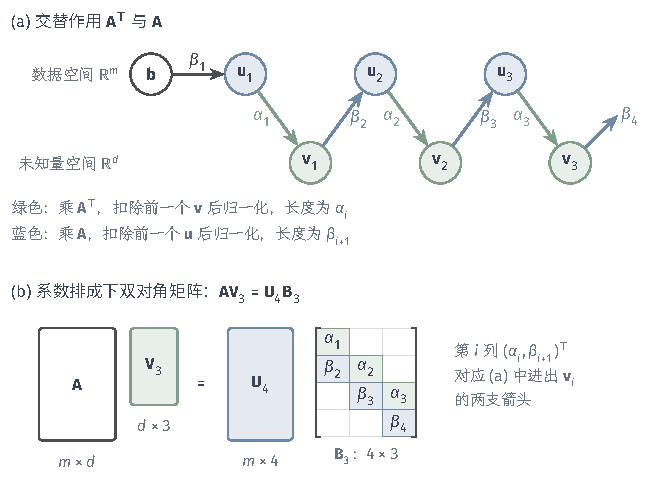
\includegraphics[width=109.343mm]{figures/01-basic-mathematics/03-vectors-matrices-and-multivariate-functions/tikz/c5-golub-kahan-bidiagonal/figure.pdf}
  \caption{Golub--Kahan双对角化的递推与矩阵关系（$k=3$）。(a)蓝色$\bm u_i$在数据空间，绿色$\bm v_i$在未知量空间；乘$\bm A^\top$并扣除前一个$\bm v$后归一化得到$\bm v_i$，长度为$\alpha_i$，乘$\bm A$并扣除前一个$\bm u$后归一化得到$\bm u_{i+1}$，长度为$\beta_{i+1}$。(b)这些长度排成$4\times3$的下双对角矩阵$\bm B_3$，满足$\bm A\bm V_3=\bm U_4\bm B_3$；绿格为对角元，蓝格为次对角元，其余元素为零。}
  \label{fig:ls-golub-kahan-bidiagonal}
\end{figure}

\paragraph{数值稳定性}
在浮点运算中，正交性所依赖的相消只近似成立，短递推也不会去掉舍入引入的旧方向分量，两组基会逐渐失去正交性；它对求解结果的影响交给两种求解器，由第~\ref{sec:ls-krylov-stopping}节的真实残差复核来控制。

\paragraph{计算代价}
每轮至多一次$\bm A$乘向量和一次$\bm A^\top$乘向量，外加两次向量更新、两次范数和两次缩放。LSQR与LSMR只用当前的$\bm u_k,\bm v_k$，不保存整组基、不作完整再正交化时，工作存储为$O(m+d)$。双对角化只负责生成候选空间，收敛快慢取决于下一步在子空间中怎样选取近似解。

\subsection{LSQR算法}
\label{sec:ls-lsqr}

\subsubsection{主要思想}

LSQR由Paige与Saunders提出\scite{math-paige1982lsqr}，它在$\operatorname{range}(\bm V_k)$中直接最小化原残差。令$\bm x=\bm V_k\bm y$，由$\bm b=\beta_1\bm u_1=\bm U_{k+1}\beta_1\bm e_1$和\eqref{eq:ls-golub-kahan-relations}，
\[
 \bm b-\bm A\bm V_k\bm y=\bm U_{k+1}(\beta_1\bm e_1-\bm B_k\bm y).
\]
$\bm U_{k+1}$的列标准正交，不改变长度，所以第$k$步只需解一个$(k+1)\times k$的双对角最小二乘问题：
\begin{equation}
 \bm x_k=\bm V_k\bm y_k,\qquad
 \bm y_k=\argmin_{\bm y\in\mathbb R^k}\lVert\beta_1\bm e_1-\bm B_k\bm y\rVert_2 .
 \label{eq:ls-lsqr-subproblem}
\end{equation}
这一做法不要求$\bm A$是方阵、满秩或相容，相容方程与不相容最小二乘问题都适用。$\bm B_k$每轮只多一行一列，小问题的QR分解可以用一次新的Givens旋转延续下去，解也随之用短递推更新。

\subsubsection{算法实现}

\paragraph{初始化}
LSQR的输入是一般的实矩阵$\bm A$与$\bm b$，允许秩亏，输出为$\bm x$。超参数是阈值和步数上限$K$：以最小二乘为目标时，用正规残差的绝对阈值$\tau_n\ge0$；以相容方程为目标时，另用第~\ref{sec:ls-stationary-stopping}节的$\mathrm{atol},\mathrm{rtol}$。初值固定为$\bm x_0=\bm0$。若$K=0$，直接输出$\bm x_0$；否则先按第~\ref{sec:ls-krylov-stopping}节检查初值。初值的原残差是$\bm b$，正规残差$\bm A^\top\bm b$的长度是$\alpha_1\beta_1$，这一检查与双对角化的起步共用同一次$\bm A^\top$乘法。初值已满足条件或起步给出零解时输出$\bm x_0$，否则取
\[
 \bm w_1=\bm v_1,\qquad \bar\rho_1=\alpha_1,\qquad \bar\phi_1=\beta_1 .
\]
这里$\bar\rho_1$是小问题第一列尚未旋转的对角元，$\bar\phi_1$是右端$\beta_1\bm e_1$的第一个分量，$\bm w_1$是第一个更新方向。

\paragraph{双对角化与Givens旋转}
第$k$轮先做一次双对角化，得到$\beta_{k+1},\alpha_{k+1}$及存在的$\bm u_{k+1},\bm v_{k+1}$。此前的旋转已把小问题的前$k-1$行化为上三角形；第$k$、$k+1$两行待处理的是第$k$列的$(\bar\rho_k,\beta_{k+1})$、新的第$k+1$列的$(0,\alpha_{k+1})$和右端的$(\bar\phi_k,0)$。按第~\ref{sec:ls-gmres}节的旋转约定，取一次Givens旋转消去$\beta_{k+1}$：
\[
 \rho_k=\sqrt{\bar\rho_k^2+\beta_{k+1}^2},\qquad
 c_k=\frac{\bar\rho_k}{\rho_k},\qquad s_k=\frac{\beta_{k+1}}{\rho_k}.
\]
同一旋转作用于新列和右端，得到
\[
 \begin{gathered}
 \theta_{k+1}=s_k\alpha_{k+1},\qquad
 \bar\rho_{k+1}=c_k\alpha_{k+1},\\
 \phi_k=c_k\bar\phi_k,\qquad
 \bar\phi_{k+1}=-s_k\bar\phi_k .
 \end{gathered}
\]
其中$\rho_k$与$\theta_{k+1}$是上双对角因子$\bm R_k$的新对角元和上对角元，$\phi_k$是变换后右端的第$k$个分量，$\bar\rho_{k+1}$与$\bar\phi_{k+1}$留给下一轮。

\paragraph{更新解与停止}
旋转完成后，用当前方向更新解：
\[
 \bm x_k=\bm x_{k-1}+\frac{\phi_k}{\rho_k}\bm w_k .
\]
这时原残差与正规残差的长度可以直接从标量读出，分别为$|\bar\phi_{k+1}|$和$|\bar\phi_{k+1}|\alpha_{k+1}|c_k|$。若相应的估计达到第~\ref{sec:ls-krylov-stopping}节的阈值，或已达到$K$，就按该节复核后输出$\bm x_k$；否则取下一方向$\bm w_{k+1}=\bm v_{k+1}-(\theta_{k+1}/\rho_k)\bm w_k$，进入下一轮。$\bm w_{k+1}$排在$\bm x_k$之后计算，因为两者都要用旧的$\bm w_k$。双对角化出现零系数时，本轮的旋转和解更新照常完成，之后不再生成下一方向：$\beta_{k+1}=0$使$s_k=0$，原残差估计为零；$\alpha_{k+1}=0$使正规残差估计为零。正常步骤中$\rho_k>0$：$\bar\rho_1=\alpha_1>0$，而只要继续迭代就有$\alpha_{k+1}>0$，归纳可知各$\bar\rho_k\ne0$，所以$\rho_k\ge|\bar\rho_k|>0$。

\begin{example}[直线拟合上的LSQR]
\label{ex:ls-lsqr-line}
沿用示例~\ref{ex:ls-golub-kahan-line}的系数。初始化取$\bm w_1=\bm v_1$、$\bar\rho_1=\alpha_1\approx2.6034$、$\bar\phi_1=3$。第一轮的旋转由$(\bar\rho_1,\beta_2)\approx(2.6034,0.5944)$得$\rho_1\approx2.6704$、$c_1\approx0.9749$、$s_1\approx0.2226$；作用于新列和右端，得$\theta_2\approx0.1658$、$\bar\rho_2\approx0.7259$、$\phi_1\approx2.9247$、$\bar\phi_2\approx-0.6678$。更新解得
\[
 \bm x_1=\frac{\phi_1}{\rho_1}\bm w_1=\frac{61}{435}(5,6)^\top\approx(0.7011,0.8414)^\top ,
\]
它是沿$\bm A^\top\bm b=(5,6)^\top$方向使残差最小的点。两个估计$|\bar\phi_2|\approx0.6678$和$|\bar\phi_2|\alpha_2|c_1|\approx0.4848$与直接计算的$\lVert\bm b-\bm A\bm x_1\rVert_2=\sqrt{194/435}$和$\lVert\bm A^\top(\bm b-\bm A\bm x_1)\rVert_2$一致。由于$\alpha_3=0$，第二轮完成旋转和更新后结束：$\rho_2\approx0.9173$、$\phi_2\approx-0.5285$，$\bm w_2=\bm v_2-(\theta_2/\rho_1)\bm w_1\approx(-0.8080,0.5925)^\top$，$\bm x_2=\bm x_1+(\phi_2/\rho_2)\bm w_2=(7/6,1/2)^\top$，正是最小二乘解$\hat{\bm x}$；原残差估计$|\bar\phi_3|\approx0.4082=1/\sqrt6$等于最优残差$(-1/6,1/3,-1/6)^\top$的长度，正规残差估计为零。
\end{example}

\subsubsection{算法分析}

\paragraph{正确性}
先说明递推确实解出了小问题\eqref{eq:ls-lsqr-subproblem}。

\begin{theorem}[LSQR递推的正确性]
\label{thm:ls-lsqr-recursion}
在精确算术中，设双对角化在第$k$轮之前没有终止。则按上述递推得到的$\bm x_k$等于$\bm V_k\bm y_k$，其中$\bm y_k$是小问题\eqref{eq:ls-lsqr-subproblem}的解，即$\bm x_k$是$\operatorname{range}(\bm V_k)$中使$\lVert\bm b-\bm A\bm x\rVert_2$最小的点；并且
\[
 \lVert\bm r_k\rVert_2=|\bar\phi_{k+1}|,\qquad
 \lVert\bm A^\top\bm r_k\rVert_2=|\bar\phi_{k+1}|\,\alpha_{k+1}|c_k| .
\]
\end{theorem}

\begin{proof}
记前$k$次旋转之积为$\bm Q_k$。每轮的新列只在第$k$、$k+1$行非零，此前的旋转都不触及它的第$k+1$行，所以一次新旋转就能延续三角化，归纳得到
\[
 \bm Q_k\begin{bmatrix}\bm B_k&\beta_1\bm e_1\end{bmatrix}
 =\begin{bmatrix}\bm R_k&\bm f_k\\ \bm0^\top&\bar\phi_{k+1}\end{bmatrix},
\]
其中$\bm R_k$上双对角，对角元为$\rho_1,\ldots,\rho_k$，上对角元为$\theta_2,\ldots,\theta_k$，$\bm f_k=(\phi_1,\ldots,\phi_k)^\top$。$\bm Q_k$正交，所以$\lVert\beta_1\bm e_1-\bm B_k\bm y\rVert_2^2=\lVert\bm f_k-\bm R_k\bm y\rVert_2^2+\bar\phi_{k+1}^2$，最小点是$\bm y_k=\bm R_k^{-1}\bm f_k$，最小残差$|\bar\phi_{k+1}|$就是$\lVert\bm r_k\rVert_2$。把$\bm V_k\bm R_k^{-1}$的第$i$列记作$\bm w_i/\rho_i$，比较$(\bm V_k\bm R_k^{-1})\bm R_k=\bm V_k$的各列，即得$\bm w_{i+1}=\bm v_{i+1}-(\theta_{i+1}/\rho_i)\bm w_i$；$\bm R_k$和$\bm f_k$在后续轮次中不再改动，回代因此化为逐步累加$\bm x_k=\bm x_{k-1}+\phi_k\bm w_k/\rho_k$。正规残差估计来自\eqref{eq:ls-golub-kahan-relations}的第二式：小问题的残差$\bm g_k=\beta_1\bm e_1-\bm B_k\bm y_k$满足$\bm B_k^\top\bm g_k=\bm0$，所以$\bm A^\top\bm r_k=\alpha_{k+1}(\bm e_{k+1}^\top\bm g_k)\bm v_{k+1}$，而$\bm e_{k+1}^\top\bm g_k=c_k\bar\phi_{k+1}$。
\end{proof}

\paragraph{残差的单调性与选出的解}
由此可以读出LSQR的几条性质。候选空间逐轮嵌套，所以精确算术中原残差不增；正规残差没有这样的保证，可能某一步上升。每个$\bm v_i$都由$\bm A^\top$作用后再作组合得到，零初值使各步近似都留在$\operatorname{range}(\bm A^\top)$中。一旦达到正规方程，$\bm x_k$就是与$\operatorname{null}(\bm A)$正交的最小二乘解，即第~\ref{sec:ls-pseudoinverse}节的$\bm A^\dagger\bm b$；$\alpha_{k+1}=0$正是这种情形。

\paragraph{与正规方程上CG的关系}
LSQR与正规方程上的CG还有下面的等价关系。

\begin{theorem}[LSQR与正规方程上的CG]
\label{thm:ls-lsqr-cg-equivalence}
在精确算术中，只要两种方法都尚未终止，LSQR的第$k$步近似就等于对正规方程$\bm A^\top\bm A\bm x=\bm A^\top\bm b$从$\bm x_0=\bm0$施行第~\ref{sec:ls-conjugate-gradient}节CG的第$k$步近似。
\end{theorem}

\begin{proof}
记$\hat{\bm x}=\bm A^\dagger\bm b$，$\hat{\bm r}=\bm b-\bm A\hat{\bm x}$。CG的各步都在$\mathcal K_k(\bm A^\top\bm A,\bm A^\top\bm b)\subseteq\operatorname{range}(\bm A^\top)$中，$\bm A^\top\bm A$在这个子空间上正定，所以CG的第$k$步是该Krylov空间中使$\lVert\bm x-\hat{\bm x}\rVert_{\bm A^\top\bm A}^2=\lVert\bm A(\bm x-\hat{\bm x})\rVert_2^2$最小的点。另一方面，$\hat{\bm r}$与$\operatorname{range}(\bm A)$正交，由勾股定理
\[
 \lVert\bm b-\bm A\bm x\rVert_2^2=\lVert\hat{\bm r}\rVert_2^2+\lVert\bm A(\bm x-\hat{\bm x})\rVert_2^2 ,
\]
右边第一项与$\bm x$无关。由定理~\ref{thm:ls-golub-kahan-relations}，两种方法的候选空间都是$\operatorname{range}(\bm V_k)$，最小化的又是同一个函数；$\bm A$在$\operatorname{range}(\bm A^\top)$上是单射，最小点唯一，所以两者相等。
\end{proof}

\paragraph{收敛速度与数值敏感度}
由这一等价，CG的收敛界可以直接搬到LSQR：迭代面对的是$\bm A^\top\bm A$，收敛快慢由$\bm A$的非零奇异值的平方的分布决定。$\bm A$满列秩时，$\kappa_2(\bm A^\top\bm A)=\kappa_2(\bm A)^2$，CG界中的$\sqrt{\kappa}$正好是$\kappa_2(\bm A)$，于是$\lVert\bm A(\bm x_k-\hat{\bm x})\rVert_2\le2\bigl((\kappa_2(\bm A)-1)/(\kappa_2(\bm A)+1)\bigr)^k\lVert\bm A\hat{\bm x}\rVert_2$。LSQR不形成Gram矩阵，避免了第~\ref{sec:ls-normal-equations-method}节在形成$\bm A^\top\bm A$时丢失信息，但这并不消除原问题的病态性：$\kappa_2(\bm A)$很大时上式的因子仍接近$1$，问题对数据的敏感度也不因算法改变。有限精度下基的正交性和两个残差估计都会偏离精确值，仍须按第~\ref{sec:ls-krylov-stopping}节复核。

\paragraph{计算代价}
每轮的核心工作是一次$\bm A$乘向量和一次$\bm A^\top$乘向量，另加十几次标量运算、一次旋转和两次长度为$d$的向量更新；需要保存的是$\bm u$和$\bm v,\bm w,\bm x$，工作存储为$O(m+d)$。

\subsection{LSMR算法}
\label{sec:ls-lsmr}

\subsubsection{主要思想}

LSMR由Fong与Saunders提出\scite{math-fong2011lsmr}。它与LSQR在同一个子空间$\operatorname{range}(\bm V_k)$中取点，但改为最小化正规残差$\lVert\bm A^\top(\bm b-\bm A\bm x)\rVert_2$，这正是判断是否到达最小二乘解所看的量。用$\bm A^\top$左乘原残差的表示$\bm U_{k+1}(\beta_1\bm e_1-\bm B_k\bm y)$，由\eqref{eq:ls-golub-kahan-relations}的第二式及$\bm B_k^\top\bm e_1=\alpha_1\bm e_1$、$\bm e_{k+1}^\top\bm B_k=\beta_{k+1}\bm e_k^\top$，得到
\begin{equation}
 \begin{gathered}
 \bm A^\top(\bm b-\bm A\bm V_k\bm y)
 =\bm V_{k+1}\bigl(\alpha_1\beta_1\bm e_1-\overline{\bm T}_k\bm y\bigr),\\
 \overline{\bm T}_k=\begin{bmatrix}\bm B_k^\top\bm B_k\\ \alpha_{k+1}\beta_{k+1}\bm e_k^\top\end{bmatrix}.
 \end{gathered}
 \label{eq:ls-lsmr-subproblem}
\end{equation}
$\bm V_{k+1}$的列标准正交，所以第$k$步求解小问题$\min_{\bm y}\lVert\alpha_1\beta_1\bm e_1-\overline{\bm T}_k\bm y\rVert_2$。实际计算不形成$\bm B_k^\top\bm B_k$，否则又回到了Gram矩阵；LSMR用两组旋转逐层处理双对角系数，同样不形成$\bm A^\top\bm A$。

\subsubsection{算法实现}

\paragraph{初始化}
输入、超参数、零初值和输出的约定都与LSQR相同。按双对角化起步并检查初值，零解直接输出；否则取
\[
 \begin{gathered}
 \bm x_0=\bm0,\qquad \bm h_1=\bm v_1,\qquad \bar{\bm h}_0=\bm0,\\
 \bar\alpha_1=\alpha_1,\qquad \bar\zeta_1=\alpha_1\beta_1,\\
 \rho_0=\bar\rho_0=1,\qquad \bar c_0=1,\qquad \bar s_0=0 .
 \end{gathered}
\]
$\bar\zeta_1=\lVert\bm A^\top\bm b\rVert_2$是初始正规残差的长度；$\bar\alpha_1$相当于LSQR中的$\bar\rho_1$，改名是为了把带横线的$\rho$留给第二组旋转。其余几个量只是占位，使第一轮的公式不必单独处理：$\bar s_0=0$使第一轮的$\bar\theta_1=0$，$\bar{\bm h}_0=\bm0$使$\bar{\bm h}_1=\bm h_1$。

\paragraph{第一组旋转}
第$k$轮先完成一次双对角化，再作第一组旋转。它与LSQR的旋转相同，把$\bm B_k$化为上双对角因子$\bm R_k$：
\[
 \begin{gathered}
 \rho_k=\sqrt{\bar\alpha_k^2+\beta_{k+1}^2},\qquad
 c_k=\frac{\bar\alpha_k}{\rho_k},\qquad s_k=\frac{\beta_{k+1}}{\rho_k},\\
 \theta_{k+1}=s_k\alpha_{k+1},\qquad
 \bar\alpha_{k+1}=c_k\alpha_{k+1}.
 \end{gathered}
\]

\paragraph{第二组旋转}
接着作第二组旋转。它处理的是对角元为$\rho_i$、下对角元为$\theta_{i+1}$的下双对角矩阵，新列在第$k$、$k+1$行上的元素是$\rho_k,\theta_{k+1}$。上一轮的旋转$(\bar c_{k-1},\bar s_{k-1})$先作用于这一列的第$k-1$、$k$行，在第$k-1$行产生$\bar\theta_k$，在第$k$行留下$\bar c_{k-1}\rho_k$；本轮旋转再消去它下方的$\theta_{k+1}$，并把右端分量$\bar\zeta_k$分成$\zeta_k$与留给下一轮的$\bar\zeta_{k+1}$：
\[
 \begin{gathered}
 \bar\theta_k=\bar s_{k-1}\rho_k,\qquad
 \bar\rho_k=\sqrt{(\bar c_{k-1}\rho_k)^2+\theta_{k+1}^2},\\
 \bar c_k=\frac{\bar c_{k-1}\rho_k}{\bar\rho_k},\qquad
 \bar s_k=\frac{\theta_{k+1}}{\bar\rho_k},\\
 \zeta_k=\bar c_k\bar\zeta_k,\qquad
 \bar\zeta_{k+1}=-\bar s_k\bar\zeta_k .
 \end{gathered}
\]
第二组旋转用到本轮的$\rho_k,\theta_{k+1}$，所以排在第一组之后。

\paragraph{更新方向与解}
两组旋转完成后，先形成第二层方向，再更新解：
\[
 \bar{\bm h}_k=\bm h_k-\frac{\bar\theta_k\rho_k}{\rho_{k-1}\bar\rho_{k-1}}\bar{\bm h}_{k-1},
 \qquad
 \bm x_k=\bm x_{k-1}+\frac{\zeta_k}{\rho_k\bar\rho_k}\bar{\bm h}_k .
\]
$|\bar\zeta_{k+1}|$是当前正规残差长度的估计。以最小二乘为目标时，它达到第~\ref{sec:ls-krylov-stopping}节的阈值或已达到$K$，就按该节复核后输出$\bm x_k$；以相容方程为目标时，递推不直接给出原残差，在候选终止处由$\bm b-\bm A\bm x_k$计算。未结束时取下一方向$\bm h_{k+1}=\bm v_{k+1}-(\theta_{k+1}/\rho_k)\bm h_k$。两组方向都使用当前的$\bm h_k$，所以$\bm h_{k+1}$放在最后计算。双对角化出现零系数时，本轮的两组旋转和解更新照常完成，然后结束：$\alpha_{k+1}=0$（含$\beta_{k+1}=0$时的约定）使$\theta_{k+1}=0$、$\bar s_k=0$，于是$\bar\zeta_{k+1}=0$。正常步骤中$\rho_k,\bar\rho_k$都为正，理由与LSQR中的$\rho_k$相同。

\subsubsection{算法分析}

\paragraph{正确性}
两组旋转对应两层三角分解，由此可以把LSMR的最优性与它和MINRES的关系一并写出。

\begin{theorem}[LSMR的最小正规残差性及与MINRES的等价]
\label{thm:ls-lsmr-minres-equivalence}
在精确算术中，设双对角化在第$k$轮之前没有终止。则LSMR递推得到的$\bm x_k$是$\operatorname{range}(\bm V_k)=\mathcal K_k(\bm A^\top\bm A,\bm A^\top\bm b)$中使正规残差$\lVert\bm A^\top(\bm b-\bm A\bm x)\rVert_2$最小的唯一点，最小值为$|\bar\zeta_{k+1}|$；它也等于对正规方程$\bm A^\top\bm A\bm x=\bm A^\top\bm b$从$\bm x_0=\bm0$施行第~\ref{sec:ls-minres}节MINRES的第$k$步近似，即该Krylov空间中使$\lVert\bm A^\top\bm b-\bm A^\top\bm A\bm x\rVert_2$最小的点。
\end{theorem}

\begin{proof}
由\eqref{eq:ls-lsmr-subproblem}及$\bm V_{k+1}$的列标准正交，$\bm x=\bm V_k\bm y$的正规残差长度等于$\lVert\alpha_1\beta_1\bm e_1-\overline{\bm T}_k\bm y\rVert_2$，只需说明递推解出了这个小问题。第一组旋转给出$\bm B_k=\bm Q_k^\top[\bm R_k;\bm0^\top]$，所以$\bm B_k^\top\bm B_k=\bm R_k^\top\bm R_k$；又$\theta_{k+1}\rho_k=\alpha_{k+1}\beta_{k+1}$，而$\bm R_k$的末行是$\rho_k\bm e_k^\top$，于是
\[
 \overline{\bm T}_k=\begin{bmatrix}\bm R_k^\top\\ \theta_{k+1}\bm e_k^\top\end{bmatrix}\bm R_k .
\]
左边的因子是下双对角的，形状与$\bm B_k$相同。$\bm R_k$的对角元$\rho_i$都为正，换元$\bm t=\bm R_k\bm y$是可逆的；第二组旋转像LSQR一样把左边的因子化为上双对角因子$\bar{\bm R}_k$（对角元$\bar\rho_i$，上对角元$\bar\theta_{i+1}$）和右端$\bm z_k=(\zeta_1,\ldots,\zeta_k)^\top$，最小残差为$|\bar\zeta_{k+1}|$。因此
\[
 \bm x_k=\bm V_k\bm R_k^{-1}\bar{\bm R}_k^{-1}\bm z_k .
\]
$\bm V_k\bm R_k^{-1}$的第$i$列是$\bm h_i/\rho_i$，与LSQR的$\bm w_i$相同；再右乘$\bar{\bm R}_k^{-1}$，第$i$列成为$\bar{\bm h}_i/(\rho_i\bar\rho_i)$，逐列比较即得$\bar{\bm h}_k$的递推，而$\bm z_k$的分量此后不再改变，所以解按$\bm x_k=\bm x_{k-1}+\zeta_k\bar{\bm h}_k/(\rho_k\bar\rho_k)$累加。两套方向正来自这两层三角求解。

最小点唯一，是因为$\operatorname{range}(\bm V_k)\subseteq\operatorname{range}(\bm A^\top)$，而$\operatorname{null}(\bm A^\top\bm A)=\operatorname{null}(\bm A)$与$\operatorname{range}(\bm A^\top)$正交，$\bm x\mapsto\bm A^\top\bm A\bm x$在这个子空间上是单射。由定理~\ref{thm:ls-golub-kahan-relations}，该子空间就是$\mathcal K_k(\bm A^\top\bm A,\bm A^\top\bm b)$。对称矩阵$\bm A^\top\bm A$、右端$\bm A^\top\bm b$与零初值下，MINRES在同一个Krylov空间中最小化同一个函数$\lVert\bm A^\top\bm b-\bm A^\top\bm A\bm x\rVert_2$，所以两者的第$k$步相同。
\end{proof}

\paragraph{残差的单调性}
候选空间逐轮嵌套，所以精确算术中正规残差不增。原残差同样不增。记同一步LSQR与LSMR的近似为$\bm x_k^{\mathrm Q}$与$\bm x_k^{\mathrm M}$，可以证明后者是截至当前步各LSQR近似的凸组合，$\bm x_{k+1}^{\mathrm M}$又是$\bm x_k^{\mathrm M}$与$\bm x_{k+1}^{\mathrm Q}$的凸组合，而$\lVert\bm b-\bm A\bm x\rVert_2^2$是凸函数，且$\bm x_{k+1}^{\mathrm Q}$在包含$\bm x_k^{\mathrm M}$的空间中使它最小。

\paragraph{选出的解与收敛速度}
零初值使各步留在$\operatorname{range}(\bm A^\top)$中，与LSQR的论证相同，达到正规方程时选出$\bm A^\dagger\bm b$。由定理~\ref{thm:ls-lsmr-minres-equivalence}，在行空间上LSMR等价于正规方程上的MINRES，速度同样受非零奇异值平方的分布控制。小奇异值与正交性损失仍然影响精度；两个残差单调，并不推出解的误差也单调。

\paragraph{计算代价}
每轮的核心工作仍是一次$\bm A$乘向量和一次$\bm A^\top$乘向量。与LSQR相比，LSMR多一组标量旋转和一套方向$\bar{\bm h}_k$的更新，需要保存$\bm u$和$\bm v,\bm h,\bar{\bm h},\bm x$，工作存储仍为$O(m+d)$。

\subsection{预条件}
\label{sec:ls-preconditioning}

\subsubsection{主要思想}

前面各方法的收敛快慢由系数矩阵的谱或奇异值分布决定。预条件选一个固定的可逆矩阵$\bm M$，它在某种意义上接近$\bm A$，而$\bm M\bm z=\bm r$又容易求解；把方程改写为$\bm M^{-1}\bm A\bm x=\bm M^{-1}\bm b$或$\bm A\bm M^{-1}\bm y=\bm b$，迭代面对的就是更集中的谱分布，所需步数随之减少。实现时不显式求$\bm M^{-1}$，也不形成变换后的矩阵，每次需要时求解一次$\bm M\bm z=\bm r$。

\subsubsection{算法实现}

\paragraph{常用预条件}
预条件$\bm M$是超参数，输入仍为$\bm A,\bm b$，输出仍为$\bm x$。对角缩放取$\bm M=\operatorname{diag}(a_{1,1},\ldots,a_{d,d})$，要求对角元非零，一次应用只是逐项相除。SSOR预条件取第~\ref{sec:ls-ssor}节的分裂矩阵，$\bm A$对称正定且$0<\omega<2$时它对称正定，一次应用是一次前代、一次对角缩放和一次回代。不完全分解在第~\ref{sec:ls-lu}节的LU或第~\ref{sec:ls-cholesky}节的Cholesky消元中只保留预先指定位置上的元素，得到稀疏的近似因子，一次应用是两次稀疏三角回代。

\paragraph{PCG的初始化}
下面以预条件共轭梯度法（PCG）为例写出完整步骤。要求$\bm A$与$\bm M$都对称正定，超参数为$\bm x_0,\mathrm{atol},\mathrm{rtol},K$和$\bm M$；本小节的$\alpha_k,\beta_k,\rho_k$是CG的步长、组合系数和内积，与双对角化的系数无关。初始化时计算$\bm r_0=\bm b-\bm A\bm x_0$，并按第~\ref{sec:ls-stationary-stopping}节作停止检查；未结束时求解$\bm M\bm z_0=\bm r_0$，取$\rho_0=\bm r_0^\top\bm z_0$、$\bm p_0=\bm z_0$。

\paragraph{PCG的每轮更新}
第$k$轮先计算
\[
 \begin{gathered}
 \bm q_k=\bm A\bm p_k,\qquad \alpha_k=\frac{\rho_k}{\bm p_k^\top\bm q_k},\\
 \bm x_{k+1}=\bm x_k+\alpha_k\bm p_k,\qquad \bm r_{k+1}=\bm r_k-\alpha_k\bm q_k ,
 \end{gathered}
\]
然后按第~\ref{sec:ls-stationary-stopping}节检查，满足阈值或达到$K$时输出$\bm x$。未结束时求解$\bm M\bm z_{k+1}=\bm r_{k+1}$，再取
\[
 \rho_{k+1}=\bm r_{k+1}^\top\bm z_{k+1},\qquad
 \beta_k=\frac{\rho_{k+1}}{\rho_k},\qquad
 \bm p_{k+1}=\bm z_{k+1}+\beta_k\bm p_k .
\]
与CG相比，只是新方向由预条件残差$\bm z$而不是$\bm r$组合而成，内积$\bm r^\top\bm r$换成$\bm r^\top\bm z$。$\bm A$与$\bm M$正定保证正常步骤的两个分母为正；残差为零时已先结束。

\paragraph{其他方法中的预条件}
其他方法不必另写完整算法，只需替换系数矩阵的作用。右预条件求解$\bm A\bm M^{-1}\bm y=\bm b$，再令$\bm x=\bm M^{-1}\bm y$：例如GMRES每次需要$\bm A\bm M^{-1}\bm v$时，先解$\bm M\bm z=\bm v$再乘$\bm A$。对LSQR和LSMR，两种方法都把$\bm A\bm v$换成$\bm A(\bm M^{-1}\bm v)$，把$\bm A^\top\bm u$换成$\bm M^{-\top}(\bm A^\top\bm u)$，结束时由$\bm y$换回$\bm x$。

\begin{example}[贯穿例上的一步PCG]
\label{ex:ls-pcg-one-step}
对示例~\ref{ex:ls-stationary-running-example}的$\bm A,\bm b$与$\bm x_0=\bm0$，取对角缩放$\bm M=\operatorname{diag}(4,3)$。初始化得$\bm r_0=(1,2)^\top$，$\bm z_0=\bm M^{-1}\bm r_0=(1/4,2/3)^\top$，$\rho_0=\bm r_0^\top\bm z_0=19/12$，$\bm p_0=\bm z_0$。第一轮，$\bm q_0=\bm A\bm p_0=(5/3,9/4)^\top$，$\bm p_0^\top\bm q_0=23/12$，$\alpha_0=19/23$，于是
\[
 \bm x_1=\Bigl(\frac{19}{92},\frac{38}{69}\Bigr)^\top\approx(0.2065,0.5507)^\top,\qquad
 \bm r_1=\Bigl(-\frac{26}{69},\frac{13}{92}\Bigr)^\top ,
\]
直接计算$\bm b-\bm A\bm x_1$得到同一残差。CG最小化的误差$\lVert\bm x-\bm x_\star\rVert_{\bm A}$从初值处的$\sqrt{15/11}\approx1.168$降到约$0.236$；同一初值下普通CG的第一步是$(1/4,1/2)^\top$，这一误差约为$0.337$。再继续一轮，
\[
 \bm z_1=\Bigl(-\frac{13}{138},\frac{13}{276}\Bigr)^\top,\qquad
 \beta_0=\frac{\rho_1}{\rho_0}=\frac{169}{6348},\qquad
 \alpha_1=\frac{276}{209},
\]
得到$\bm x_2=(1/11,7/11)^\top=\bm x_\star$，与二维问题至多两步结束一致。
\end{example}

\subsubsection{算法分析}

\paragraph{正确性}
PCG的正确性来自一个保持对称的变换。取$\bm M=\bm C\bm C^\top$，令$\widehat{\bm A}=\bm C^{-1}\bm A\bm C^{-\top}$，它对称正定。下面的定理说明，PCG就是对$\widehat{\bm A}$施行CG后换回原变量。

\begin{theorem}[PCG与变换后CG的等价]
\label{thm:ls-pcg-equivalence}
设$\bm A,\bm M$对称正定，$\bm M=\bm C\bm C^\top$，$\widehat{\bm A}=\bm C^{-1}\bm A\bm C^{-\top}$。在精确算术中，只要PCG尚未终止，它的迭代量与对$\widehat{\bm A}\bm y=\bm C^{-1}\bm b$从$\bm y_0=\bm C^\top\bm x_0$施行CG所得的迭代量满足
\[
 \bm y_k=\bm C^\top\bm x_k,\qquad \hat{\bm r}_k=\bm C^{-1}\bm r_k,\qquad \hat{\bm p}_k=\bm C^\top\bm p_k .
\]
因此$\bm x_k$是$\bm x_0+\mathcal K_k(\bm M^{-1}\bm A,\bm M^{-1}\bm r_0)$中使$\lVert\bm x-\bm x_\star\rVert_{\bm A}$最小的唯一点，并且
\[
 \begin{gathered}
 \lVert\bm x_k-\bm x_\star\rVert_{\bm A}\le2\Bigl(\frac{\sqrt{\hat\kappa}-1}{\sqrt{\hat\kappa}+1}\Bigr)^k\lVert\bm x_0-\bm x_\star\rVert_{\bm A},\\
 \hat\kappa=\kappa_2(\widehat{\bm A})=\frac{\lambda_{\max}(\bm M^{-1}\bm A)}{\lambda_{\min}(\bm M^{-1}\bm A)} .
 \end{gathered}
\]
\end{theorem}

\begin{proof}
对$k$归纳。$k=0$时，$\hat{\bm r}_0=\bm C^{-1}\bm b-\widehat{\bm A}\bm C^\top\bm x_0=\bm C^{-1}\bm r_0$，$\hat{\bm p}_0=\hat{\bm r}_0=\bm C^\top(\bm C^{-\top}\bm C^{-1}\bm r_0)=\bm C^\top\bm z_0=\bm C^\top\bm p_0$。设第$k$步对应关系成立，则
\[
 \hat{\bm r}_k^\top\hat{\bm r}_k=\bm r_k^\top\bm M^{-1}\bm r_k=\bm r_k^\top\bm z_k,\qquad
 \hat{\bm p}_k^\top\widehat{\bm A}\hat{\bm p}_k=\bm p_k^\top\bm A\bm p_k ,
\]
两种方法的步长相同，于是$\bm y_{k+1}=\bm C^\top\bm x_{k+1}$，$\hat{\bm r}_{k+1}=\bm C^{-1}(\bm r_k-\alpha_k\bm A\bm p_k)=\bm C^{-1}\bm r_{k+1}$；组合系数同为$\rho_{k+1}/\rho_k$，故$\hat{\bm p}_{k+1}=\bm C^{-1}\bm r_{k+1}+\beta_k\bm C^\top\bm p_k=\bm C^\top(\bm z_{k+1}+\beta_k\bm p_k)=\bm C^\top\bm p_{k+1}$。

由定理~\ref{thm:ls-cg-convergence}，$\bm y_k$是$\bm y_0+\mathcal K_k(\widehat{\bm A},\hat{\bm r}_0)$中使$\lVert\bm y-\bm C^\top\bm x_\star\rVert_{\widehat{\bm A}}$最小的唯一点。换回$\bm x=\bm C^{-\top}\bm y$时，$\lVert\bm C^\top(\bm x-\bm x_\star)\rVert_{\widehat{\bm A}}=\lVert\bm x-\bm x_\star\rVert_{\bm A}$，且$\bm C^{-\top}\widehat{\bm A}^j\hat{\bm r}_0=(\bm M^{-1}\bm A)^j\bm M^{-1}\bm r_0$，所以仿射子空间和目标都对应过来，收敛界也随之成立。最后，$\bm M^{-1}\bm A=\bm C^{-\top}\widehat{\bm A}\bm C^\top$与$\widehat{\bm A}$相似，而$\widehat{\bm A}$对称正定，$\kappa_2(\widehat{\bm A})$就是特征值之比。
\end{proof}

$\bm M^{-1}\bm A$本身一般不对称，不能直接交给普通CG；定理中的$\bm C$只用于论证，算法只需求解$\bm M\bm z=\bm r$。论证要求整个迭代使用同一个固定的线性作用$\bm M^{-1}$；预条件随轮次变化时，标准PCG的共轭性与最优性不再沿用。

\paragraph{收敛速度}
定理把速度归结为$\bm M^{-1}\bm A$的特征值分布。对角缩放适合各行各列尺度相差很大的矩阵。例如取$d=10$，$\bm A=\bm S\bm T\bm S$，其中$\bm S=\operatorname{diag}(1,2,\ldots,10)$，$\bm T$是对角元为$1$、次对角元为$0.4$的三对角矩阵。$\bm A$的对角部分是$\bm S^2$，取$\bm M=\bm S^2$与$\bm C=\bm S$，变换后恰好$\widehat{\bm A}=\bm T$，特征值为$1+0.8\cos(j\pi/11)$，$j=1,\ldots,10$。图~\ref{fig:ls-preconditioned-spectrum}比较两组特征值：$\bm A$的特征值从约$0.73$铺到约$133$，比值约$182.7$；缩放后全部落在$[0.23,1.77]$内，比值约$7.61$。定理中的收缩因子相应从约$0.862$降到约$0.468$，而每轮只多一次逐项除法。

\begin{figure}[htbp]
  \centering
  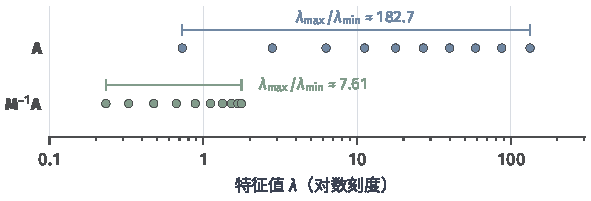
\includegraphics[width=100mm]{figures/01-basic-mathematics/03-vectors-matrices-and-multivariate-functions/matplotlib/c5-preconditioned-spectrum/figure.pdf}
  \caption{对角缩放前后的特征值分布（对数横轴）。矩阵为$\bm A=\bm S\bm T\bm S$，$\bm S=\operatorname{diag}(1,\ldots,10)$，$\bm T$为对角元$1$、次对角元$0.4$的三对角矩阵，预条件$\bm M=\operatorname{diag}(\bm A)$。蓝点为$\bm A$的$10$个特征值（数值计算），绿点为$\bm M^{-1}\bm A$的特征值$1+0.8\cos(j\pi/11)$；括线标出各自的范围与最大、最小特征值之比。}
  \label{fig:ls-preconditioned-spectrum}
\end{figure}

\paragraph{计算代价}
每轮比CG多一次$\bm M$求解，选用时要同时计入构造$\bm M$与每轮应用的成本，比较达到同一精度的总工作量。

\paragraph{GMRES与MINRES的预条件}
对GMRES，左预条件在预条件后的Krylov空间中最小化$\lVert\bm M^{-1}(\bm b-\bm A\bm x)\rVert_2$，右预条件保留原残差$\lVert\bm b-\bm A\bm x\rVert_2$作为目标；两者结束时都回到第~\ref{sec:ls-stationary-stopping}节检查原残差。MINRES要求保持对称性，只能采用对称正定预条件$\bm M=\bm C\bm C^\top$的分裂变换$\bm C^{-1}\bm A\bm C^{-\top}$。预条件只改善变换后的谱，不改变原问题对数据的敏感度。

\paragraph{最小二乘目标的保持}
对不相容最小二乘问题，还要核对变换是否保持原目标。左变换给出$\lVert\bm M^{-1}(\bm b-\bm A\bm x)\rVert_2^2=(\bm b-\bm A\bm x)^\top\bm M^{-\top}\bm M^{-1}(\bm b-\bm A\bm x)$，即第~\ref{sec:ls-weighted-ls}节以$\bm M^{-\top}\bm M^{-1}$为权的加权目标，一般会改变解。可逆右变换$\bm x=\bm M^{-1}\bm y$使两个问题的残差逐点相同，原残差目标和解集都保留；但零初值在$\bm y$坐标下选出的是$\lVert\bm y\rVert_2=\lVert\bm M\bm x\rVert_2$最小的解，秩亏时它未必是原坐标下欧氏范数最小的最小二乘解。

\subsection{收敛检验与停止准则}
\label{sec:ls-krylov-stopping}

方阵上的CG、PCG、GMRES、MINRES、BiCG与BiCGSTAB统一沿用第~\ref{sec:ls-stationary-stopping}节的规则：超参数为$\bm x_0,\mathrm{atol},\mathrm{rtol},K$，以$\tau=\mathrm{atol}+\mathrm{rtol}\lVert\bm b\rVert_2$检查真实原残差$\lVert\bm b-\bm A\bm x_k\rVert_2$，达到阈值或步数上限时输出当前$\bm x$。达到上限本身不表示已经收敛。递推残差和小问题残差只用于内部计算，决定何时值得复核，不另作算法输出。

LSQR与LSMR以相容方程为目标时，可以沿用同一原残差阈值。以最小二乘为目标时，不相容问题的最优原残差不为零，原残差阈值可能永远达不到，所以单列非负超参数$\tau_n$，检查
\[
 \lVert\bm A^\top(\bm b-\bm A\bm x_k)\rVert_2\le\tau_n ,
\]
允许原残差非零。$\tau_n$是绝对阈值，应与所用数据的尺度相配，不除以$\lVert\bm A^\top\bm b\rVert_2$这类可能为零的参照量。初值已满足条件时直接输出$\bm x_0=\bm0$；其余情况在每次候选终止和最终输出前，都用$\bm A,\bm b,\bm x_k$重新计算残差复核。达到$K$时只输出当前$\bm x$，残差和停止原因都不纳入输出。

残差小的含义还要结合原问题的条件数来解释；要求最小范数解时，还须保持零初值、迭代留在行空间，并核对预条件下的选解准则。真实残差复核所需的矩阵乘法计入实际成本。误差的解释留到第~\ref{sec:ls-numerical-sensitivity}节，达到同一精度的综合比较留到第~\ref{sec:ls-method-selection}节。
